\documentclass{article}

\usepackage{siunitx}
\usepackage{graphicx}
\usepackage{tikz}
\usepackage{pgfplots}
\usepackage{amsmath}
\pgfplotsset{compat=1.18}

\begin{document}
    \section{Breve repaso}
        El exerimento de Young consiste en hacer insidir un 
        frente de onda plano (caracterizado por 
        una longitud de onda y una frecuencia) a traves
        de una pantalla óptica con 2 rendijas 
        de grosor $a$, que se separan una distancia $d$.
        Lo que se quiere es observar el efecto de puntos $p$
        lejanos que se encuentran a una distancia $L_0$ con
        la caracteristica de
        \begin{math}
            L_0 >> d >> a
        \end{math}

        Se otiene que el efecto neto en el punto $p$ está
        dado por:

        

        \[
            \psi(p) = A(\delta)\sin(wt-\gamma)
        \]

        Donde:\\

        \(A(\delta) = E_{A}\cos(\frac{k\delta}{2})\)\\ 

        \(\gamma = kx + \frac{k\delta}{2} + \pi\)\\

        \begin{center}
            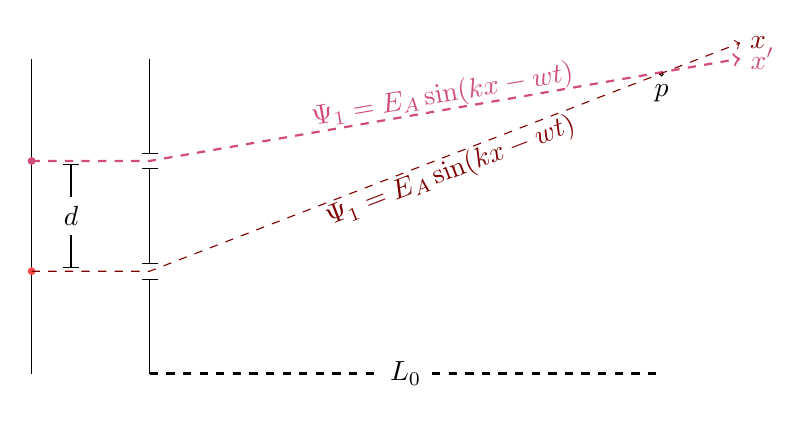
\begin{tikzpicture}[transform shape, scale=1]
                \draw (0,0) -- (0,4);
                \draw (1.5,0) -- (1.5,1.2);
                \draw (1.5,4) -- (1.5,2.8);
                \draw (1.5,2.6) -- (1.5,1.4);
                \draw (1.4,2.8) -- (1.6,2.8);
                \draw (1.4,2.6) -- (1.6,2.6);
                \draw (1.4,1.4) -- (1.6,1.4);
                \draw (1.4,1.2) -- (1.6,1.2);
                \draw[thick, dashed] (1.5,0) -- (8,0) node[midway,fill = white]{$L_0$};
                \draw (8,3.8) circle (0.2mm) node[below]{$p$};
                \fill[purple! 70! white] (0,2.7) circle (0.5mm);
                \fill[red! 70! white] (0,1.3) circle (0.5mm);

                \draw[purple!70!,thick,dashed, ->] (0,2.7) -- (1.5,2.7) -- 
                node[midway, yshift=1.8mm, sloped]{$\Psi_1 = E_A \sin(kx - wt)$} (9,4) node[right] {$x'$};

                \draw[color=red!50!black,dashed, ->] (0,1.3) -- (1.5,1.3) --
                node[midway, yshift=-2mm, sloped] 
                {$\Psi_1 = E_A \sin(kx - wt)$} (9,4.2) node[right] {$x$};

                \draw (0.5,1.35) -- (0.5,2.65) node [midway, fill=white]{$d$};
                \draw (0.4,1.35) -- (0.6,1.35);
                \draw (0.4,2.65) -- (0.6,2.65);
                
            \end{tikzpicture}
        \end{center}

        Recordemos que la energía que transporta una onda electromagnética
        está dada por el vector de Poynting, cuya magnitud es la intensidad
        \((\frac{watts}{\si{\meter\squared}})\) 
        \[\vec{S} = \frac{\vec{E} \times \vec{B}}{\mu_0}\]
        Donde $\mu_0 = 4\pi \times 10^{-7} \unit[per-mode = symbol]{\T\meter\per\ampere}$

        \begin{itemize}
            \item Propiedades de las ondas electromagnéticas
            \subitem $\vec{E} \perp \vec{B}$
            \subitem $E = cB$ donde $c$ es la velocidad de 
            la rediación en el vacío
        \end{itemize}

        Por lo que se tiene que
        \[\vec{S} = \frac{\vec{E} \times \vec{B}}{\mu_0} = 
        \frac{E^2}{c\mu_0} \widehat{\perp} = \frac{cB^2}{\mu_0} \widehat{\perp}\]
        
        con $\widehat{\perp}$ siendo la dirección perpendicular 
        al plano que contiene a $\vec{E}$ y a $\vec{B}$. 
        De esta forma si \(\psi(p) = E(p) = A(\delta)\sin(wt-\gamma)\),
        entonces 
        \[S = \frac{(A(\delta))^2\sin^2(wt-\gamma)}{c\mu_0}\] 
        y la intensidad romedio en el tiempo está dada por 

        \begin{eqnarray}
            \langle S \rangle_T &=& 
            \frac{1}{T}\int_{0}^{T} S(t)dt \\
            &=& \frac{1}{T}\int_{0}^{T}\frac{(A(\delta))^2\sin^2(wt-\gamma)}
            {c\mu_0}dt \\
            &=& \frac{(A(\delta))^2}{2c\mu_0}\\
            &=& \frac{4E_A^2\cos(\frac{k\delta}{2})}{2c\mu_0}\\
            &=& I_{nmax}\cos^2(\frac{k\delta}{2})
        \end{eqnarray}

        \section{Rendija Ancha}



        ESPACIO PARA GRAFIQUITAS

        Cuando se tiene una rendija ancha, y se hace insidir 
        un frente de onda plano, provoca que cada punto del 
        frente de onda sea un emisor isotrópico de ondas, cuyo 
        efecto neto es la superposición de todas las ondas que
        llegan a un punto $p$.

        Por el principio de super posición, se tendrá que el efecto
        neto será dado por:
        \begin{eqnarray}
            \psi(P) &=& 
            \psi_0 + \psi_1 + ... + \psi_N \\
            &=& \sum_{i=0}^{N} \psi_i \\
            &=& \sum_{i=0}^{N} E_A\sin(kx - wt + ik\delta) 
        \end{eqnarray}
        donde $ik\delta$ es el valor de desfase respecto a $\psi_0$
         y $\delta = \Delta y \sin(\theta)$

        Para poder calcular el valor de la sumatoria primero 
        reescribimos $\psi_0$:

        \begin{eqnarray}
            \psi(P) &=& E_A\sin(kx-wt) \\
            &=& E_A\sin(wt - kx + \pi) \\
            &=& E_A\sin(wt+\gamma) 
        \end{eqnarray}

        con $\gamma = \pi - kx$ 
    
        Luego, definimos el fasor $\psi_{f0}$ como un vector que
        va rotando a una frecuencia angular $w$ y tamaño $E_A$

        \begin{center}
            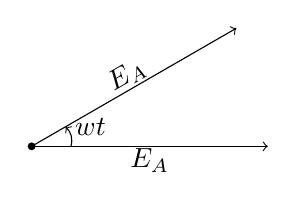
\begin{tikzpicture}
                \fill (0,0) circle (0.5mm);
                \draw[->] (0,0) -- (3,0) node[midway, yshift=-1.8mm, sloped ]{$E_A$};
                \draw[->] (0,0) -- (2.6,1.5)  node[midway, yshift=1.8mm, sloped]{$E_A$};
                \draw[ -> ] (0.5,0) to [bend right] (0.43, 0.25) node[right] {$wt$};
            \end{tikzpicture}
        \end{center}

        Si sumamos 2 fasores $\psi_0$ y $\psi_1$ de tamaño $E_A$, $\psi_1$ desfazado
        un ángulo $k\delta$ con respecto a  $\psi_0$, entonces se consigue un
        fasor resultante de magnitud $E_R$

        \begin{center}
            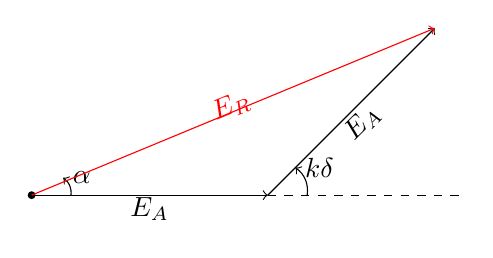
\begin{tikzpicture}
                \fill (0,0) circle (0.5mm);
                \draw[->] (0,0) -- (3,0) node[midway, yshift=-1.8mm, sloped ]{$E_A$};
                \draw[->] (3,0) -- (5.12,2.12)  node[midway, yshift=-2mm, sloped]{$E_A$};
                \draw[dashed] (3,0) -- (5.5,0);
                \draw[ -> ] (0.5,0) to [bend right] (0.40, 0.22) node[right] {$\alpha$};
                \draw[red! 100!,->] (0,0) -- (5.12,2.12) node[midway, yshift=2, sloped]{$E_R$};
                \draw[ -> ] (3.5,0) to [bend right] (3.35, 0.35) node[right] {$k\delta$};
            \end{tikzpicture}
        \end{center}

        Cuando N tiende a infinito, el tamaño del fasor y el desfase
        entre fasores tiende a un diferencial. De esta manera, la curva
        que describen los fasores tiende a un arco de circunferencia.

        \begin{center}
            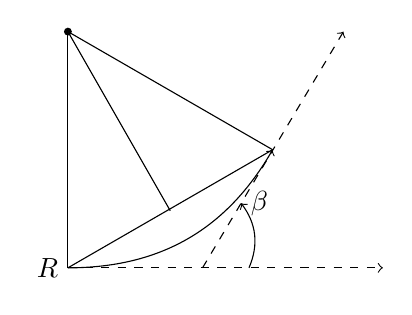
\begin{tikzpicture}
                \fill (0,3) circle (0.5mm);
                \draw (0,3) -- (0,0) node[left, sloped ]{$R$};
                \draw (0,0) -- (2.6,1.5);
                \draw (0,3) -- (2.6,1.5);
                \draw[ -> ] (0,0) to [bend right] (2.6, 1.5);
                \draw[dashed, ->] (0,0) -- (4,0);
                \draw[ -> ] (2.3,0) to [bend right] (2.2, 0.82) node[right] {$\beta$};
                \draw (0,3) -- (1.3,0.725);
                \draw[dashed, ->] (1.71,0) -- (3.5,3);
            \end{tikzpicture}
        \end{center}

        Nota: el ángulo que se forma entre los dos vertices de tamaño $R$ también es $\beta$ 

        Donde:
        \begin{eqnarray}
            \beta &=& Nk\delta \\
            &=& N\frac{2\pi}{\lambda}\Delta y \sin(\theta) \\
            &=& \frac{2\pi a \sin(\theta)}{\lambda} 
        \end{eqnarray}
        y se obtiene que:
        \[\sin(\frac{\beta}{2}) = \frac{\frac{E_{AR}}{2}}{f_eR}\]
        siendo $f_e$ un factor de escala asociado al tamaño 
        del fasor que permite poner la razón en unidades de campo

        Podemos ver que 
        \[R\beta = S\]
        que si multiplicamos a ambos lados de la igualdad 
        \[f_eR\beta = f_eS\]
        y nos queda que 
        \[E_{AS} = f_eS\]
        Lo que es la suma de todas las amplitudes que constituyen el arco

        Este resultado nos da que 
        \[\frac{E_{AS}}{\beta}=f_eR\]
        Así:
        \[E_{AR} = E_{AS}\frac{\sin(\frac{\beta}{2})}{\frac{\beta}{2}}\]
        Lo que concluye que el campo electrico en este caso 
        tiene un comportamiento 
        armónico simple con la función de onda en P:

        \[E(p) = \psi(p) = 
        E_{AS}\frac{\sin(\frac{\beta}{2})}{\frac{\beta}{2}}\sin(wt+\frac{\beta}{2})
        = E_{AR}\sin(wt+\frac{\beta}{2})\]

        \section{Energía e intensidad}
        Retomando el caso de la rendija angosta, la intensidad 
        promedio en el sistema es:

        \begin{eqnarray}
            \langle S \rangle_T &=& 
            \frac{1}{T} \int_{0}^{T} S(t)dt\\
            &=& \frac{1}{T} \int_{0}^{T}
            \frac{(E_{AR})^2\sin^2(wt+\frac{\beta}{2})}{c\mu_0}dt\\
            &=& \frac{(E_{AR})^2}{2c\mu_0}\\
            &=& \frac{E_{AS}^2\sin^2(\frac{\pi a\sin(\theta)}{\lambda})}
            {2c\mu_0(\frac{\pi a \sin(\theta)}{\lambda})}\\
            &=& I_{nmax} \frac{\sin^2(\frac{\pi a \sin(\theta)}{\lambda})}
            {(\frac{\pi a \sin(\theta)}{\lambda})}    
        \end{eqnarray}


        \includegraphics[width=1\textwidth]{C:/Users/lalal/OneDrive/Documentos/Universidad/FCOP/Teoría/Captura de pantalla 2023-10-30 005623.png}
        

        








\end{document}